\section{Graph representation}
\label{sec:ftp_graph}

%\todo{Correct image to have T0m and not T0a}

As described in section \ref{sec:ftp}, a FTP instance is completely described by a structure $G =(V_c, A, T_{0}, D, TW)$. Note that the previously referenced structure requires a set of arcs $A$ connecting every pair of nodes belonging to $V_c$. Thus, it is possible to represent this information in a weight matrix, where each of its entries corresponds to a particular arc.

Since the presented formulation of the FTP wishes to addresses a real-world situation involving commercial flights, upon constructing the weight matrix, it is necessary to take the characteristics of commercial flights into account. For any pair of cities, at any given moment in time, there are several commercial flights that connect these two cities in that particular moment. These flights are denoted as a family of arcs. Given that there is a direct mapping between commercial flights and FTP arcs, then there are multiple arcs for each weight matrix entry. Moreover, a commercial flight connecting two cities, does not have a constant price over time. Thus, the value of an arc connecting two cities, varies over time. This means that a weight matrix of a FTP instance is three dimensional, with three variables $i, j, t$, where $i$ is the origin node, $j$ the destination node, and $t$ the moment in time at which the transition occurs.

In particular, it is possible to consider a weight matrix in which, for every entry, there are multiple values, corresponding to the different possible arcs for that pair of nodes and time. Consequently, accessing a particular arc requires not only the triplet $(i, j, t)$, but also some information about which particular arc to select. 

Given that the dimensions of a FTP weight matrix are considerable, considering a family of arcs for each weight matrix entry is not recommended, since it would increase the weight size even more. Instead, a pragmatic strategy is followed. Upon constructing a weight matrix for the FTP instance, the objective function is taken into account. This means that, instead of considering that there are multiple arcs for the triplet $(i, j, t)$, it is considered that there is only one: the one that has the minimum value according to the objective function. For example, if the objective function intends to minimize the total trip cost, upon constructing the weight matrix, for each family of arcs $(i, j, t)$, only the minimum cost arc would be selected. By using this strategy there is only one available arc, for each cost matrix entry, and it is the one which minimizes the objective function.

The price of a commercial flights usually depends on the cities, dates, and  direction of traversal. This means that the weight matrix of the FTP is not necessarily symmetric. Moreover, there is also no guarantee that a commercial flight between two cities exist. In fact, there are many cities which do not have a direct flight connection. Fortunately, many commercial flight providers have this into consideration, and try to establish an indirect connection between any two cities by adding connecting flights. However, this is not always the case, and it may be necessary to initialize each entry of the weight matrix to a very high value, in order to discard these non-existent flights from a possible solution.  

To conclude the analysis of the characteristics of the FTP weight matrix, it is worth mentioning that the matrix does not need to be complete, because not every arc is relevant for the construction of a solution. While it is necessary to have every arc connecting two pair of nodes belonging to the set of nodes to be visited, it is not necessary to have every arc connecting the initial and final nodes to the others. In reality, the arcs leaving from and returning to the initial and final node, respectively, are only necessary in particular moments of time. To better understand this, consider figure \ref{fig:arc_families}, which illustrates the necessary arcs to construct a solution to a FTP instance. Every arc of a FTP instance can be classified into three different groups, according to their characteristics: \textit{initial}, \textit{transition} and \textit{final} arcs.

%% ----- use this figure to explain the arc families -----
\begin{figure}[htpb]
  \centering
  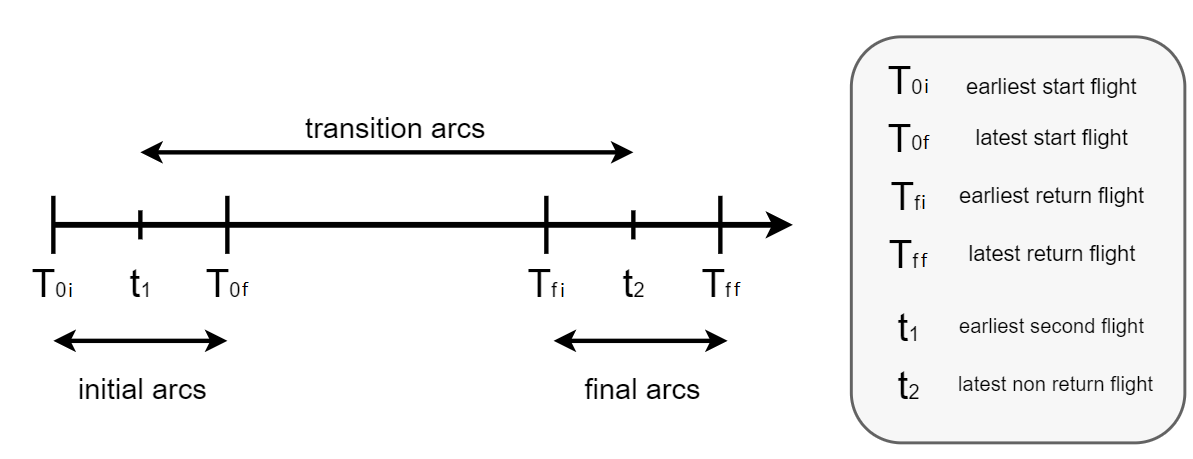
\includegraphics[width=\textwidth]{./Figures/system_design/tempos.png}
  \caption{Illustration of the distribution *in time) of the initial, final and transition arcs.}
  \label{fig:arc_families} 
\end{figure}

The \textit{initial} arcs are those which might initiate the trip. Consequently, they must start at node $v_0$, at $t \in T_0 = [T_{0m}, T_{0M}]$, connecting $v_0$ to every node in $V$. In its turn, the \textit{final} arcs are those which connect every node in $V$ to the return node, $v_{n+1}$ at $t$ \in [$T_{fm}$, $T_{fM}$], where $T_{fm}$ = $T_{0m} + \sum(D)$ and $T_{fM}$ = $T_{0M} + \sum(D)$, and $\sum(D)$ is the total trip duration. There are a total of $k_i = T_{0M} - T_{0m} + 1 = T_{fM} -T_{fm} + 1$ initial and final arc layers. In the example depicted in Figure~\ref{fig:multipartite_sol}, there is a single initial and final layer, since there is only one possible start date.

The \textit{transition} arcs are those which fully connect the $N$ nodes belonging to $V$. In the example presented in figure \ref{fig:arc_families}, the earliest transition arc occurs at a time no sooner than $t_1 = T_{0m} + min(D)$, where $min(D)$ corresponds to the lowest value of the set of durations. Hence, if the trip starts by traversing an initial arc at time $T_{0m}$, the first transition arc must only be traversed $min(D)$ time-units later. By following a similar approach, the latest transition arc can occur no latter than $t_2 = T_{0M} + \sum(D) - min(D)$. Thus, there are a total of $k_2 = t_2-t_1+1$ transition layers, and $k_2*n*(n-1)$ transition arcs.

The union of the initial, transition and final arcs gives the set $A$ of all the arcs, which may be used to construct a solution to the requested trip. 







\section{Dimensional overview}
\label{sec:dimensions}

This section 
%will make a brief analysis of the dimensions associated to this problem. This will cover 
presents a brief analysis of the weight matrix dimensions of an FTP instance, in particular, the number of entries and its size in memory. It also includes an overview of the solution space associated to a FTP request. 

The FTP is described by a tri-dimensional array (weight matrix), with shape $(|Vc|,|Vc|, |T_{0}| + \sum D)$, where $V_c$ is the complete set of nodes (note that$|Vc|=(n+2)$), and $T_{0}$ is the length of the start period and $\sum D$ is the total trip duration. The total number of entries ($n_e$) of the weight matrix is given by $n_{e} = (n+2)^2\times(T_{0} + \sum D)$. 

Consequently, the total number of entries of the weight matrix depends mostly on the number of cities to visit, since there is a quadratic relation. Furthermore, it is always true that $1 \leq (T_{0} + \sum D) \leq 365$, since commercial flights are not sold with more than one year in advance. Thus, it is possible to simplify the expression of the number of entries of a weight matrix by considering $n_{e} = k(n+2)^2$, where $k$ is 
$(T_{0} + \sum D)$.
%a constant - the maximum length (in days) of a possible trip schedule. 

Each entry of the weight matrix shall be represented with a 32bit integer (as described in section \ref{sec:os_implementation}) and thus, it is possible to calculate the size of the weight matrix in memory ($m_{graph}$), given by $m_{graph} = 4*n_e$ (bytes). 


Hence, when considering a TSP instance $n$ cities to visit, there are $n!$ possible routes. The goal of the FTP is to find both the best route and schedule for a trip. Note that in a FTP problem, the trip start length is given by $T_{0}$, and thus, there are at most $T_{0}$ different possible schedules. Thus, the size of the solution space to a FTP is given by $|S| = T_{0}*n!$  

From the above, it is possible to conclude that the size of the search space of an FTP instance is closely related to that of the TSP. In particular, if there is a single start date, the size is the same. As the length of the start period increases, than so does the search space. This increase is always linear, and it is usually below 3 orders of magnitude. 

Note that the procedures considered above are only true after reducing the family of arcs into a single arc, according to the objective function, as described in the previous section. Prior to this, instead of having a single 32bit integer representing a weight matrix entry, there is a structured data object (JSON) with flight information. In general, each flight roughly occupies 3500 bytes, and there are multiple flights ($\approx$1-100) for each pair of cities, and for each date. 
%Thus, 1GB of memory allows the storage of, approximately, 300.000 commercial flights. 



% Hence, it is possible to estimate that a 1 city problem has a 36
% Hence, it is possible to create table \ref{tab:dimensions} which presents the maximum number of entries of the weight matrix, and its size in memory, for FTP instances of different sizes (1-5000 cities to visit). 


% \begin{table}[h!]
% \begin{tabular}{ccccccccc}
%  \hline
% n       & 1       & 5       & 10      & 50      & 100     & 500      & 1000     & 5000       \\ \hline
% entries & 9$*k$       & 49$*k$      & 144$*k$     & 2.704$*k$    & 10.404$*k$   & 252.004$*k$   & $\approx 10^{6}*k$  & $\approx 2.5*10^{6}*k$    \\  \hline
% memory      & 36b & 196b & 576b & 10.816b & 41.616b & 10.08MB & 40.16 MB & 1000.80016 \\  \hline
% \end{tabular}
% \end{table}

